\documentclass{standalone}
\usepackage{tikz}
\usetikzlibrary{patterns, positioning}
\usepackage[sfdefault]{ClearSans} %% option 'sfdefault' activates Clear Sans as the default text font
\usepackage[T1]{fontenc}

\begin{document}
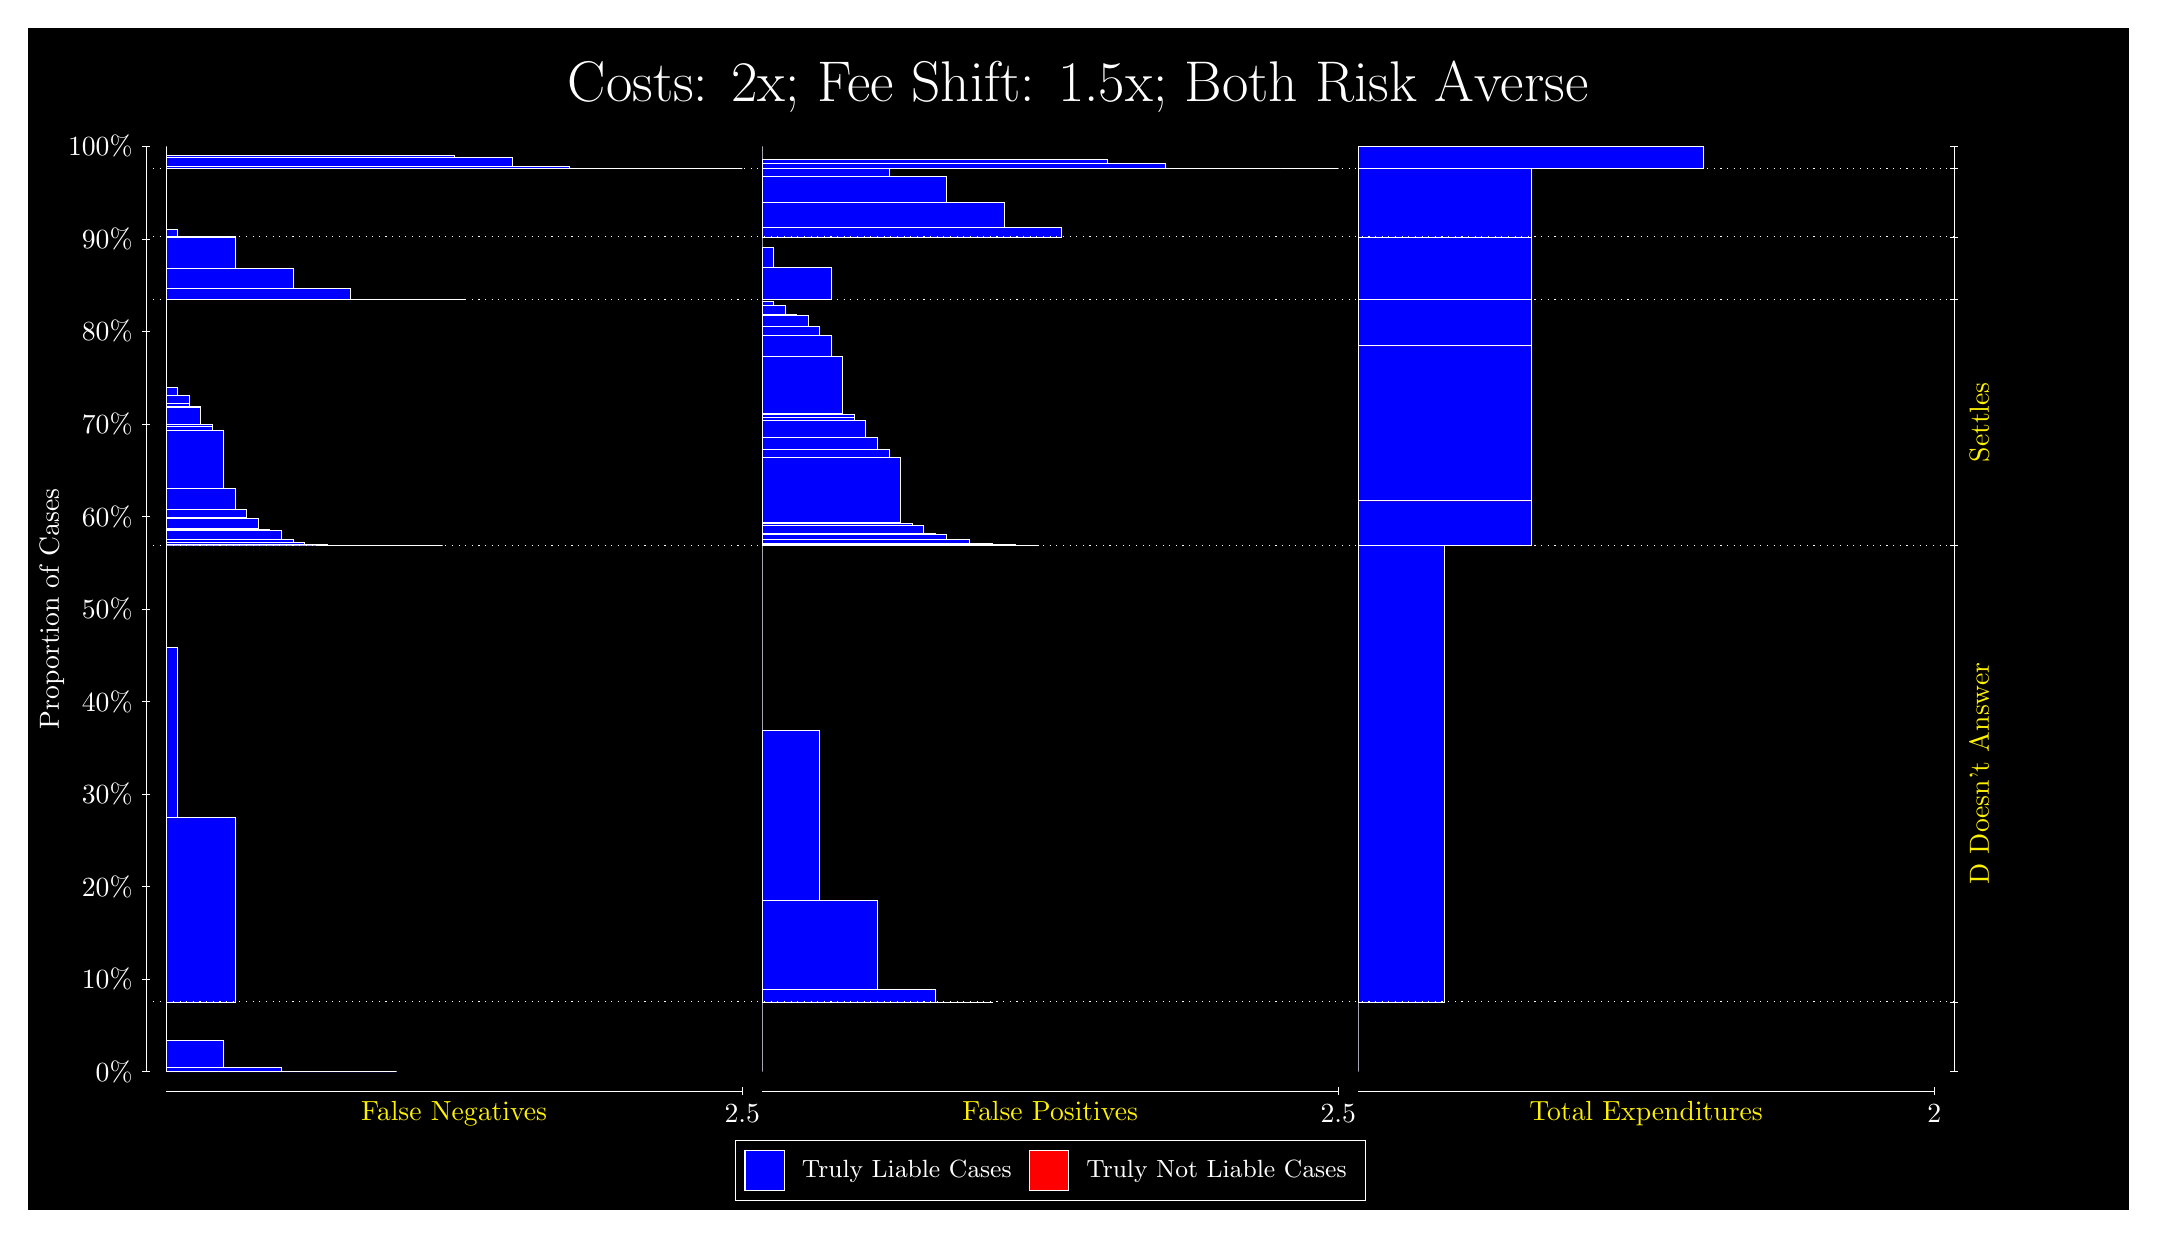
\begin{tikzpicture}
\draw[fill=black] (0,0) rectangle (26.667,15);
\draw[text=white] (0,13.5) rectangle (26.667,15) node[midway] {\huge Costs: 2x; Fee Shift: 1.5x; Both Risk Averse};
\draw[white, very thin] (1.5,1.75) -- (1.5,13.5);
\node[rotate=90, text=white, anchor=center] at (0.3, 7.625) {Proportion of Cases};
\draw[white, very thin] (1.45,1.75) -- (1.55,1.75);
\node[text=white, anchor=east] at (1.45, 1.75) {0\%};
\draw[white, very thin] (1.45,2.925) -- (1.55,2.925);
\node[text=white, anchor=east] at (1.45, 2.925) {10\%};
\draw[white, very thin] (1.45,4.1) -- (1.55,4.1);
\node[text=white, anchor=east] at (1.45, 4.1) {20\%};
\draw[white, very thin] (1.45,5.275) -- (1.55,5.275);
\node[text=white, anchor=east] at (1.45, 5.275) {30\%};
\draw[white, very thin] (1.45,6.45) -- (1.55,6.45);
\node[text=white, anchor=east] at (1.45, 6.45) {40\%};
\draw[white, very thin] (1.45,7.625) -- (1.55,7.625);
\node[text=white, anchor=east] at (1.45, 7.625) {50\%};
\draw[white, very thin] (1.45,8.8) -- (1.55,8.8);
\node[text=white, anchor=east] at (1.45, 8.8) {60\%};
\draw[white, very thin] (1.45,9.975) -- (1.55,9.975);
\node[text=white, anchor=east] at (1.45, 9.975) {70\%};
\draw[white, very thin] (1.45,11.15) -- (1.55,11.15);
\node[text=white, anchor=east] at (1.45, 11.15) {80\%};
\draw[white, very thin] (1.45,12.325) -- (1.55,12.325);
\node[text=white, anchor=east] at (1.45, 12.325) {90\%};
\draw[white, very thin] (1.45,13.5) -- (1.55,13.5);
\node[text=white, anchor=east] at (1.45, 13.5) {100\%};

\draw[white, very thin] (24.457,1.75) -- (24.457,13.5);
\draw[white, very thin] (24.407,1.75) -- (24.507,1.75);
\node[anchor=west] at (24.407, 1.75) {};
\draw[white, very thin] (24.407,2.6338) -- (24.507,2.6338);
\node[anchor=west] at (24.407, 2.6338) {};
\draw[white, very thin] (24.407,8.4337) -- (24.507,8.4337);
\node[anchor=west] at (24.407, 8.4337) {};
\draw[white, very thin] (24.407,11.56) -- (24.507,11.56);
\node[anchor=west] at (24.407, 11.56) {};
\draw[white, very thin] (24.407,12.351) -- (24.507,12.351);
\node[anchor=west] at (24.407, 12.351) {};
\draw[white, very thin] (24.407,13.219) -- (24.507,13.219);
\node[anchor=west] at (24.407, 13.219) {};
\draw[white, very thin] (24.407,13.5) -- (24.507,13.5);
\node[anchor=west] at (24.407, 13.5) {};

\draw[white, very thin, fill=blue] (1.75,1.75) rectangle (4.6775,1.75);
\draw[white, very thin, fill=blue] (1.75,1.75) rectangle (3.9457,1.7505);
\draw[white, very thin, fill=blue] (1.75,1.7505) rectangle (3.2138,1.8092);
\draw[white, very thin, fill=blue] (1.75,1.8092) rectangle (2.4819,2.143);
\draw[white, very thin, fill=red] (1.75,2.143) rectangle (1.75,2.143);
\draw[white, very thin, fill=blue] (1.75,2.143) rectangle (1.75,2.6338);
\draw[white, very thin, fill=blue] (1.75,2.6338) rectangle (2.6283,4.9818);
\draw[white, very thin, fill=blue] (1.75,4.9818) rectangle (1.8964,7.1402);
\draw[white, very thin, fill=red] (1.75,7.1402) rectangle (1.75,7.1402);
\draw[white, very thin, fill=blue] (1.75,7.1402) rectangle (1.75,8.4337);
\draw[white, very thin, fill=blue] (1.75,8.4337) rectangle (5.2631,8.4337);
\draw[white, very thin, fill=blue] (1.75,8.4337) rectangle (4.9703,8.4337);
\draw[white, very thin, fill=blue] (1.75,8.4337) rectangle (4.6775,8.4337);
\draw[white, very thin, fill=blue] (1.75,8.4337) rectangle (4.5312,8.4339);
\draw[white, very thin, fill=blue] (1.75,8.4339) rectangle (4.3848,8.4339);
\draw[white, very thin, fill=blue] (1.75,8.4339) rectangle (4.3848,8.4339);
\draw[white, very thin, fill=blue] (1.75,8.4339) rectangle (4.2384,8.4341);
\draw[white, very thin, fill=blue] (1.75,8.4341) rectangle (4.092,8.4342);
\draw[white, very thin, fill=blue] (1.75,8.4342) rectangle (3.9457,8.4363);
\draw[white, very thin, fill=blue] (1.75,8.4363) rectangle (3.7993,8.441);
\draw[white, very thin, fill=blue] (1.75,8.441) rectangle (3.6529,8.4412);
\draw[white, very thin, fill=blue] (1.75,8.4412) rectangle (3.6529,8.4452);
\draw[white, very thin, fill=blue] (1.75,8.4452) rectangle (3.5065,8.4453);
\draw[white, very thin, fill=blue] (1.75,8.4453) rectangle (3.5065,8.467);
\draw[white, very thin, fill=blue] (1.75,8.467) rectangle (3.3602,8.5085);
\draw[white, very thin, fill=blue] (1.75,8.5085) rectangle (3.2138,8.6248);
\draw[white, very thin, fill=blue] (1.75,8.6248) rectangle (3.0674,8.6306);
\draw[white, very thin, fill=blue] (1.75,8.6306) rectangle (3.0674,8.64);
\draw[white, very thin, fill=blue] (1.75,8.64) rectangle (2.921,8.6443);
\draw[white, very thin, fill=blue] (1.75,8.6443) rectangle (2.921,8.7767);
\draw[white, very thin, fill=blue] (1.75,8.7767) rectangle (2.921,8.7768);
\draw[white, very thin, fill=blue] (1.75,8.7768) rectangle (2.7746,8.786);
\draw[white, very thin, fill=blue] (1.75,8.786) rectangle (2.7746,8.8947);
\draw[white, very thin, fill=blue] (1.75,8.8947) rectangle (2.6283,9.163);
\draw[white, very thin, fill=blue] (1.75,9.163) rectangle (2.4819,9.8932);
\draw[white, very thin, fill=blue] (1.75,9.8932) rectangle (2.3355,9.9389);
\draw[white, very thin, fill=blue] (1.75,9.9389) rectangle (2.3355,9.9727);
\draw[white, very thin, fill=blue] (1.75,9.9727) rectangle (2.1891,9.9761);
\draw[white, very thin, fill=blue] (1.75,9.9761) rectangle (2.1891,10.187);
\draw[white, very thin, fill=blue] (1.75,10.187) rectangle (2.1891,10.193);
\draw[white, very thin, fill=blue] (1.75,10.193) rectangle (2.0428,10.234);
\draw[white, very thin, fill=blue] (1.75,10.234) rectangle (2.0428,10.338);
\draw[white, very thin, fill=blue] (1.75,10.338) rectangle (1.8964,10.438);
\draw[white, very thin, fill=red] (1.75,10.438) rectangle (1.75,10.438);
\draw[white, very thin, fill=blue] (1.75,10.438) rectangle (1.75,11.56);
\draw[white, very thin, fill=blue] (1.75,11.56) rectangle (5.5558,11.56);
\draw[white, very thin, fill=blue] (1.75,11.56) rectangle (4.8239,11.563);
\draw[white, very thin, fill=blue] (1.75,11.563) rectangle (4.092,11.693);
\draw[white, very thin, fill=blue] (1.75,11.693) rectangle (3.3602,11.945);
\draw[white, very thin, fill=blue] (1.75,11.945) rectangle (2.6283,12.351);
\draw[white, very thin, fill=red] (1.75,12.351) rectangle (1.75,12.351);
\draw[white, very thin, fill=blue] (1.75,12.351) rectangle (2.6283,12.353);
\draw[white, very thin, fill=blue] (1.75,12.353) rectangle (1.8964,12.451);
\draw[white, very thin, fill=red] (1.75,12.451) rectangle (1.75,12.451);
\draw[white, very thin, fill=blue] (1.75,12.451) rectangle (1.75,13.219);
\draw[white, very thin, fill=blue] (1.75,13.219) rectangle (9.0689,13.219);
\draw[white, very thin, fill=blue] (1.75,13.219) rectangle (8.337,13.219);
\draw[white, very thin, fill=blue] (1.75,13.219) rectangle (7.6051,13.221);
\draw[white, very thin, fill=blue] (1.75,13.221) rectangle (6.8732,13.249);
\draw[white, very thin, fill=blue] (1.75,13.249) rectangle (6.1413,13.363);
\draw[white, very thin, fill=blue] (1.75,13.363) rectangle (5.4094,13.384);
\draw[white, very thin, fill=blue] (1.75,13.384) rectangle (4.6775,13.384);
\draw[white, very thin, fill=blue] (1.75,13.384) rectangle (3.0674,13.384);
\draw[white, very thin, fill=blue] (1.75,13.384) rectangle (2.3355,13.384);
\draw[white, very thin, fill=red] (1.75,13.384) rectangle (1.75,13.384);
\draw[white, very thin, fill=blue] (1.75,13.384) rectangle (1.75,13.5);
\draw[white, very thin, fill=red] (9.3189,1.75) rectangle (9.3189,1.75);
\draw[white, very thin, fill=blue] (9.3189,1.75) rectangle (9.3189,2.6338);
\draw[white, very thin, fill=red] (9.3189,2.6338) rectangle (12.246,2.6338);
\draw[white, very thin, fill=blue] (9.3189,2.6338) rectangle (12.246,2.6353);
\draw[white, very thin, fill=blue] (9.3189,2.6353) rectangle (11.515,2.7943);
\draw[white, very thin, fill=blue] (9.3189,2.7943) rectangle (10.783,3.9274);
\draw[white, very thin, fill=blue] (9.3189,3.9274) rectangle (10.051,6.0857);
\draw[white, very thin, fill=blue] (9.3189,6.0857) rectangle (9.3189,8.4337);
\draw[white, very thin, fill=red] (9.3189,8.4337) rectangle (12.832,8.4337);
\draw[white, very thin, fill=blue] (9.3189,8.4337) rectangle (12.832,8.4391);
\draw[white, very thin, fill=red] (9.3189,8.4391) rectangle (12.539,8.4391);
\draw[white, very thin, fill=blue] (9.3189,8.4391) rectangle (12.539,8.444);
\draw[white, very thin, fill=red] (9.3189,8.444) rectangle (12.246,8.444);
\draw[white, very thin, fill=blue] (9.3189,8.444) rectangle (12.246,8.4542);
\draw[white, very thin, fill=blue] (9.3189,8.4542) rectangle (12.1,8.4578);
\draw[white, very thin, fill=red] (9.3189,8.4578) rectangle (11.954,8.4578);
\draw[white, very thin, fill=blue] (9.3189,8.4578) rectangle (11.954,8.5083);
\draw[white, very thin, fill=blue] (9.3189,8.5083) rectangle (11.807,8.5119);
\draw[white, very thin, fill=red] (9.3189,8.5119) rectangle (11.661,8.5119);
\draw[white, very thin, fill=blue] (9.3189,8.5119) rectangle (11.661,8.5721);
\draw[white, very thin, fill=blue] (9.3189,8.5721) rectangle (11.515,8.5834);
\draw[white, very thin, fill=red] (9.3189,8.5834) rectangle (11.368,8.5834);
\draw[white, very thin, fill=blue] (9.3189,8.5834) rectangle (11.368,8.6867);
\draw[white, very thin, fill=blue] (9.3189,8.6867) rectangle (11.222,8.7162);
\draw[white, very thin, fill=blue] (9.3189,8.7162) rectangle (11.075,8.727);
\draw[white, very thin, fill=red] (9.3189,8.727) rectangle (11.075,8.727);
\draw[white, very thin, fill=blue] (9.3189,8.727) rectangle (11.075,9.5555);
\draw[white, very thin, fill=blue] (9.3189,9.5555) rectangle (10.929,9.6555);
\draw[white, very thin, fill=red] (9.3189,9.6555) rectangle (10.783,9.6555);
\draw[white, very thin, fill=blue] (9.3189,9.6555) rectangle (10.783,9.8005);
\draw[white, very thin, fill=blue] (9.3189,9.8005) rectangle (10.636,10.021);
\draw[white, very thin, fill=red] (9.3189,10.021) rectangle (10.49,10.021);
\draw[white, very thin, fill=blue] (9.3189,10.021) rectangle (10.49,10.055);
\draw[white, very thin, fill=blue] (9.3189,10.055) rectangle (10.49,10.1);
\draw[white, very thin, fill=blue] (9.3189,10.1) rectangle (10.344,10.104);
\draw[white, very thin, fill=blue] (9.3189,10.104) rectangle (10.344,10.83);
\draw[white, very thin, fill=blue] (9.3189,10.83) rectangle (10.197,11.099);
\draw[white, very thin, fill=blue] (9.3189,11.099) rectangle (10.051,11.217);
\draw[white, very thin, fill=blue] (9.3189,11.217) rectangle (9.9044,11.353);
\draw[white, very thin, fill=blue] (9.3189,11.353) rectangle (9.758,11.363);
\draw[white, very thin, fill=blue] (9.3189,11.363) rectangle (9.758,11.369);
\draw[white, very thin, fill=blue] (9.3189,11.369) rectangle (9.6116,11.369);
\draw[white, very thin, fill=blue] (9.3189,11.369) rectangle (9.6116,11.485);
\draw[white, very thin, fill=blue] (9.3189,11.485) rectangle (9.4652,11.526);
\draw[white, very thin, fill=blue] (9.3189,11.526) rectangle (9.3189,11.56);
\draw[white, very thin, fill=red] (9.3189,11.56) rectangle (10.197,11.56);
\draw[white, very thin, fill=blue] (9.3189,11.56) rectangle (10.197,11.966);
\draw[white, very thin, fill=blue] (9.3189,11.966) rectangle (9.4652,12.218);
\draw[white, very thin, fill=blue] (9.3189,12.218) rectangle (9.3189,12.351);
\draw[white, very thin, fill=red] (9.3189,12.351) rectangle (13.125,12.351);
\draw[white, very thin, fill=blue] (9.3189,12.351) rectangle (13.125,12.478);
\draw[white, very thin, fill=blue] (9.3189,12.478) rectangle (12.393,12.79);
\draw[white, very thin, fill=blue] (9.3189,12.79) rectangle (11.661,13.119);
\draw[white, very thin, fill=blue] (9.3189,13.119) rectangle (10.929,13.218);
\draw[white, very thin, fill=blue] (9.3189,13.218) rectangle (10.197,13.219);
\draw[white, very thin, fill=red] (9.3189,13.219) rectangle (16.638,13.219);
\draw[white, very thin, fill=blue] (9.3189,13.219) rectangle (16.638,13.219);
\draw[white, very thin, fill=red] (9.3189,13.219) rectangle (15.906,13.219);
\draw[white, very thin, fill=blue] (9.3189,13.219) rectangle (15.906,13.219);
\draw[white, very thin, fill=red] (9.3189,13.219) rectangle (15.174,13.219);
\draw[white, very thin, fill=blue] (9.3189,13.219) rectangle (15.174,13.226);
\draw[white, very thin, fill=red] (9.3189,13.226) rectangle (14.442,13.226);
\draw[white, very thin, fill=blue] (9.3189,13.226) rectangle (14.442,13.281);
\draw[white, very thin, fill=blue] (9.3189,13.281) rectangle (13.71,13.33);
\draw[white, very thin, fill=blue] (9.3189,13.33) rectangle (12.978,13.336);
\draw[white, very thin, fill=blue] (9.3189,13.336) rectangle (12.246,13.336);
\draw[white, very thin, fill=blue] (9.3189,13.336) rectangle (11.515,13.336);
\draw[white, very thin, fill=red] (9.3189,13.336) rectangle (9.9044,13.336);
\draw[white, very thin, fill=blue] (9.3189,13.336) rectangle (9.9044,13.336);
\draw[white, very thin, fill=red] (9.3189,13.336) rectangle (9.3189,13.336);
\draw[white, very thin, fill=blue] (9.3189,13.336) rectangle (9.3189,13.5);
\draw[white, very thin, fill=red] (16.888,1.75) rectangle (16.888,1.75);
\draw[white, very thin, fill=blue] (16.888,1.75) rectangle (16.888,2.6338);
\draw[white, very thin, fill=red] (16.888,2.6338) rectangle (17.986,2.6338);
\draw[white, very thin, fill=blue] (16.888,2.6338) rectangle (17.986,8.4337);
\draw[white, very thin, fill=red] (16.888,8.4337) rectangle (19.083,8.4337);
\draw[white, very thin, fill=blue] (16.888,8.4337) rectangle (19.083,8.9986);
\draw[white, very thin, fill=red] (16.888,8.9986) rectangle (19.083,8.9986);
\draw[white, very thin, fill=blue] (16.888,8.9986) rectangle (19.083,10.968);
\draw[white, very thin, fill=red] (16.888,10.968) rectangle (19.083,10.968);
\draw[white, very thin, fill=blue] (16.888,10.968) rectangle (19.083,11.56);
\draw[white, very thin, fill=red] (16.888,11.56) rectangle (19.083,11.56);
\draw[white, very thin, fill=blue] (16.888,11.56) rectangle (19.083,12.351);
\draw[white, very thin, fill=red] (16.888,12.351) rectangle (19.083,12.351);
\draw[white, very thin, fill=blue] (16.888,12.351) rectangle (19.083,13.219);
\draw[white, very thin, fill=red] (16.888,13.219) rectangle (21.279,13.219);
\draw[white, very thin, fill=blue] (16.888,13.219) rectangle (21.279,13.5);
\draw[white, dotted] (1.5,2.6338) -- (24.457,2.6338);
\draw[white, dotted] (1.5,8.4337) -- (24.457,8.4337);
\draw[white, dotted] (1.5,11.56) -- (24.457,11.56);
\draw[white, dotted] (1.5,12.351) -- (24.457,12.351);
\draw[white, dotted] (1.5,13.219) -- (24.457,13.219);
\draw[white, very thin] (1.75,1.5) -- (9.0689,1.5);
\node[text=yellow, anchor=north] at (5.4094, 1.5) {False Negatives};
\draw[white, very thin] (9.0689,1.45) -- (9.0689,1.55);
\node[text=white, anchor=north] at (9.0689, 1.45) {2.5};

\draw[white, very thin] (9.3189,1.5) -- (16.638,1.5);
\node[text=yellow, anchor=north] at (12.978, 1.5) {False Positives};
\draw[white, very thin] (16.638,1.45) -- (16.638,1.55);
\node[text=white, anchor=north] at (16.638, 1.45) {2.5};

\draw[white, very thin] (16.888,1.5) -- (24.207,1.5);
\node[text=yellow, anchor=north] at (20.547, 1.5) {Total Expenditures};
\draw[white, very thin] (24.207,1.45) -- (24.207,1.55);
\node[text=white, anchor=north] at (24.207, 1.45) {2};


\node[text=yellow, centered, rotate=90] at (24.777, 5.5338) {D Doesn't Answer};
\node[text=yellow, centered, rotate=90] at (24.777, 9.9967) {Settles};




\draw (12.978300999999998,1.5) node[draw=none] (baseCoordinate) {};
\begin{scope}[align=center]
        \matrix[scale=0.5, draw=white, below=0.5cm of baseCoordinate, nodes={draw}, column sep=0.1cm]{
            \node[rectangle, draw, minimum width=0.5cm, minimum height=0.5cm, fill=blue] {}; &
            \node[draw=none, font=\small, text=white] (B) {Truly Liable Cases}; &
            \node[rectangle, draw, minimum width=0.5cm, minimum height=0.5cm, fill=red] {}; &
            \node[draw=none, font=\small, text=white] (B) {Truly Not Liable Cases}; \\
            };
\end{scope}

\end{tikzpicture}
\end{document}